% ----------------------------------------------------------------------
\title{PIBIC}
\documentclass[
	% -- opções da classe memoir --
	article,			% indica que é um artigo acadêmico
	12pt,				% tamanho da fonte
	oneside,			% para impressão apenas no verso. Oposto a twoside
	a4paper,			% tamanho do papel. 
	% -- opções da classe abntex2 --
	%chapter=TITLE,		% títulos de capítulos convertidos em letras maiúsculas
	%section=TITLE,		% títulos de seções convertidos em letras maiúsculas
	%subsection=TITLE,	% títulos de subseções convertidos em letras maiúsculas
	%subsubsection=TITLE % títulos de subsubseções convertidos em letras maiúsculas
	% -- opções do pacote babel --
	english,			% idioma adicional para hifenização
	brazil,				% o último idioma é o principal do documento
	]{abntex2}


% ---
% PACOTES
% ---

% ---
% Pacotes fundamentais 
% ---
\usepackage{cmap}				% Mapear caracteres especiais no PDF
\usepackage{lmodern}			% Usa a fonte Latin Modern
\usepackage[T1]{fontenc}		% Selecao de codigos de fonte.
\usepackage[utf8]{inputenc}		% Codificacao do documento (conversão automática dos acentos)
\usepackage{indentfirst}		% Indenta o primeiro parágrafo de cada seção.
\usepackage{nomencl} 			% Lista de simbolos
\usepackage{color}				% Controle das cores
\usepackage{graphicx}			% Inclusão de gráficos
\usepackage{pdfpages}           %i Inclui páginas de PDFs
\usepackage{amssymb}
\usepackage[svgnames]{xcolor}
\usepackage{listings}
\usepackage{amsmath}

% ---
% Configurar R code
\lstset{language=R,
    basicstyle=\small\ttfamily,
    stringstyle=\color{DarkGreen},
    otherkeywords={0,1,2,3,4,5,6,7,8,9},
    morekeywords={TRUE,FALSE},
    deletekeywords={data,frame,length,as,character},
    keywordstyle=\color{blue},
    commentstyle=\color{DarkGreen},
}
% ---
% Pacotes adicionais, usados apenas no âmbito do Modelo Canônico do abnteX2
% ---
\usepackage{lipsum}				% para geração de dummy text
% ---
		
% ---
% Pacotes de citações
% ---
\usepackage[brazilian,hyperpageref]{backref}	 % Paginas com as citações na bibl
\usepackage[alf]{abntex2cite}	% Citações padrão ABNT
% ---

% ---
% Configurações do pacote backref
% Usado sem a opção hyperpageref de backref
\renewcommand{\backrefpagesname}{Citado na(s) página(s):~}
% Texto padrão antes do número das páginas
\renewcommand{\backref}{}
% Define os textos da citação
\renewcommand*{\backrefalt}[4]{
	\ifcase #1 %
		Nenhuma citação no texto.%
	\or
		Citado na página #2.%
	\else
		Citado #1 vezes nas páginas #2.%
	\fi}%
% ---

% ---
% Informações de dados para CAPA e FOLHA DE ROSTO
% ---
\titulo{Agregação de Preferências Eleitorais via Escalagem Psicométrica de Thurstone}
\autor{Lucas Loureiro Lino da Costa}
\local{Brasil}
\data{Julho, 2018}
% ---

% ---
% Configurações de aparência do PDF final

% alterando o aspecto da cor azul
\definecolor{blue}{RGB}{41,5,195}

% informações do PDF
\makeatletter
\hypersetup{
     	%pagebackref=true,
		pdftitle={\@title}, 
		pdfauthor={\@author},
    	pdfsubject={Artigo Ciêntífico},
	    pdfcreator={LaTeX with abnTeX2},
		pdfkeywords={Agregação de Preferências Coletivas}{Escalagem Psicométrica Unidimencional} {Método de Thurstone}{Eleições Brasileiras 2018},
		colorlinks=true,       		% false: boxed links; true: colored links
    	linkcolor=blue,          	% color of internal links
    	citecolor=blue,        		% color of links to bibliography
    	filecolor=magenta,      		% color of file links
		urlcolor=blue,
		bookmarksdepth=4
}
\makeatother
% --- 

% ---
% compila o indice
% ---
\makeindex
% ---

% ---
% Altera as margens padrões
% ---
\setlrmarginsandblock{4cm}{4cm}{*}
\setulmarginsandblock{4cm}{4cm}{*}
\checkandfixthelayout
% ---

% --- 
% Espaçamentos entre linhas e parágrafos 
% --- 

% O tamanho do parágrafo é dado por:
\setlength{\parindent}{1.3cm}

% Controle do espaçamento entre um parágrafo e outro:
\setlength{\parskip}{0.2cm}  % tente também \onelineskip

% Espaçamento simples
\SingleSpacing

% ----
% Início do documento
% ----
\begin{document}

% Retira espaço extra obsoleto entre as frases.
\frenchspacing 

% ----------------------------------------------------------
% ELEMENTOS PRÉ-TEXTUAIS
% ----------------------------------------------------------

%---
%
% Se desejar escrever o artigo em duas colunas, descomente a linha abaixo
% e a linha com o texto ``FIM DE ARTIGO EM DUAS COLUNAS''.
% \twocolumn[    		% INICIO DE ARTIGO EM DUAS COLUNAS
%
%---
% página de titulo
\maketitle
% ----------------------------------------------------------
% resumo em português
% ----------------------------------------------------------
\begin{resumoumacoluna}
 Nesse trabalho utilizaremos um método incomum de lidar com dados categóricos ordinais às ciências econômicas, o método de escalagem psicométrica de Thurstone. Usar-lo-emos para determinação de preferências agregadas sobre candidatos em eleições a partir de manifestações individuais sobre pares de alternativas. Como instância de aplicação do método, tomaremos uma lista plausível de candidatos para a eleição presidencial brasileira de 2018, assim como uma amostra representativa da Faculdade de Economia, Administração, Contabilidade e Gestão de Políticas Públicas da Universidade de Brasília, para assim inferirmos as preferências coletivas da população em questão.
 
 \vspace{\onelineskip}
 
 \noindent
 \textbf{Palavras-chave}: Agregação de Preferências Coletivas. Escalagem Psicométrica Unidimensional. Método de Thurstone. Eleições Brasileiras 2018.
 
 \vspace{\onelineskip}
 
 \noindent
 \textbf{Keywords}: Collectives Aggregated Preferences. Unidimensional Psychometric Scale. Thurstone's method. Brazilian's Election 2018.
 
 \end{resumoumacoluna}

% ]  				% FIM DE ARTIGO EM DUAS COLUNAS
% ---

% ----------------------------------------------------------
% ELEMENTOS TEXTUAIS
% ----------------------------------------------------------
\textual

% ----------------------------------------------------------
% Introdução
% ----------------------------------------------------------
\section{Introdução}


O Método de Escalagem Psicométrica de Thurstone é uma ferramenta utilizada para estimação de preferências entre objetos via frequência observada dos pares comparados, \citeonline{thurstone1927law}, entretanto a sua utilização dentro do campo da Ciência Econômica ainda é escassa, sendo utilizada normalmente ferramentas de inferência econométricas no seu lugar. A fim de preencher essa lacuna epistemológica usar-mos-ei o modelo padrão de escalagem psicométrica unidimensional de Thurstone para elucidar as preferências coletivas ordinais de uma amostra de votantes. Para tanto, vamos utilizar a linguagem de programação \textit{opensource} \citeonline{EmptyId_R} para compilar e analisar os dados da pesquisa, assim como disponibilizaremos publicamente tanto o código fonte construído para tal (Anexo B), assim como, os dados da pesquisa no repositório online do autor, \citeonline{Lucas2018}. Na sessão 2 temos a definição da amostra utilizada durante a análise. Na sessão 3 é apresentado o método de escalagem psicométrica unidimensional, referindo-se a \citeonline{borg2005modern} para escalagem multidimensional e \citeonline{souza1988metodos} para apresentação de variedades de métodos de escalagem unidimensional e  multidimensional. A sessão 4 refere-se a aplicação do modelo de escalagem psicométrica unidimensional de Thurstone na amostra populacional. E finalmente a sessão 5 conclui este trabalho. 



% ----------------------------------------------------------
% Seção de explicações da Amostra
% ----------------------------------------------------------
\section{Definição da amostra}


A Faculdade de Economia, Administração, Contabilidade e Gestão de Políticas Públicas da Universidade de Brasília (FACE), segundo último anuário estatístico, publicado pelo Decanato de Planejamento, Orçamento e Avaliação Institucional, apresentava em seu quadro 2.958 alunos de graduação regulares ativos registrados no segundo semestre de 2016, \citeonline{anuariounb}\footnote{Por carácter de simplificação, tomaremos que a população se manteve estática até o período da análise, o primeiro semestre de 2018.} .

Utilizando-se do método de amostragem aleatória simples sem repetição, com a captura dos dados realizado via formulário preenchido pelos participantes do estudo (Anexo A), assim como, tomando como base um erro amostral padrão de 5\% e um nível de confiança também padrão de 95\%, temos que o tamanho mínimo da nossa amostra para que seja considerada representativa deve ser de 341 participantes, condição a qual foi saciada devido a amostra utilizada conter 360 participantes.


% ----------------------------------------------------------
% Seção do Método de Escalagem Psicométrica 
% ----------------------------------------------------------
\section{O método de escalagem psicométrica}


Segundo o método de escalagem psicométrica unidimensional de Thurstone, quando um indivíduo se depara com um conjunto de escolhas, ele individualmente designa um valor dentro de uma escala para cada alternativa. Entretanto cada designação dentro da escala é por natureza uma variável aleatória. O processo de designação dos valores adentra o que os psicólogos chamam de \textit{psychological continuum}, onde a construção da escala é oriunda de uma sub-divisão finita deste último, composto por sub-intervalos. Quando o  valor dessa variável aleatória cai sobre um dos sub-intervalos do \textit{psychological continuum}, é essa posição do sub-intervalo que determina a resposta do indivíduo a pergunta. Resposta esta categórica e ordenada da menor para a maior dentro do espectro. Ou seja, quando economistas falam sobre utilidade e psicometristas falam de escala de valores, eles estão ambos falando sobre a mesma coisa.

Considerando um conjunto finito $\mathbf{\Gamma = \{A_1, A_2, ... , A_\textit{n} \}}$ de \textit{n} diferentes candidatos, além disso supondo que cada eleitor tenha suas relações de preferência estritas $\succ$ em \textbf{X}, ou seja, completas, transitivas e anti-reflexivas nas suas relações binárias $\succ$ sobre o conjunto de candidatos em \textbf{X}.
 O eleitor designa para cada candidato $\mathbf{A_\textit{i}}$ um número real $\mu_\textit{i}$ chamado de escala de valor, ou utilidade, de $\mathbf{A_\textit{i}}$, de maneira que $\mathbf{A_\textit{i} \succ A_\textit{j}}$ se, e somente se, $\mu_\textit{i} > \mu_\textit{j}$, para $\textit{i} \neq \textit{j}$ e $\textit{i}, \textit{j} = 1, ... , \textit{n}$.
 O valor de escala $\mu_\textit{i}$ é representado por uma variável aleatória distribuída normalmente $\mathbf{X_\textit{i}}\sim N(\mu_\textit{i}, \,\sigma^2_\textit{i})$, onde a $\mu_\textit{i} \in \mathbb{R}$ e variância  $\sigma^2_\textit{i} > 0$. Dado que um grande número de eleitores independentemente designa valores de escala para um candidato, podemos assumir, pela Lei dos Números Grandes, que a media de $\mu_\textit{i}$ é uma aproximação consistente para o verdadeiro valor de escala $\mu_\textit{i}$ atribuído coletivamente para o candidato $\mathbf{A_\textit{i}}$. A suposição de normalidade é aceitável se um grande número de eleitores independentes é assumido.

Apesar dos eleitores agirem independentemente, assume-se que as variáveis aleatórias são correlatas. Onde, $\sigma_\textit{i,j} = cov(X_\textit{i}, \, X_\textit{j})$ é a covariância entre $X_\textit{i}$ e $X_\textit{j}$ e sendo $p_\textit{ij} =  \frac{\sigma_\textit{ij}}{\sigma_\textit{i} \sigma_\textit{j}}$ o coeficiente de correlação entre 
$X_\textit{i}$ e $X_\textit{j}$, exatamente pelo fato que $p_\textit{ij} \neq 0$, para $\textit{i} \neq \textit{j}$ e $\textit{i}, \textit{j} = 1, ... , \textit{n}$. Como correlação entre diferentes alternativas estão presentes no modelo, o Axioma de Interdependência das Alternativas Irrelevantes de Arrow, \citeonline{arrow2012social}, não se aplica, assim como demonstrado por \citeonline{tanguiane2012aggregation}, exatamente pelo fato deste ser uma construção meramente algébrica e não estatística. Sendo assim, por consequência o Teorema de impossibilidade de Arrow também não é válido.

Devido a aleatoriedade do processo de escalagem psicométrica, a noção de preferência é substituída pela de probabilidade de preferência. Onde $\phi_\textit{ij} = Prob[A_\textit{i} \ \succ A_\textit{j}]$ seja a probabilidade que $A_\textit{i}$ seja preferido a $A_\textit{j}$, ou seja, $\phi_\textit{ij} = Prob[X_\textit{i} \ > X_\textit{j}]$. Como variáveis aleatórias distribuídas normalmente são contínuas, definimos 
$\phi_\textit{ij} = Prob[X_\textit{i} \ \geq X_\textit{j}]$. O processo de normalização do evento $[X_\textit{i} \geq X_\textit{j}]$ é demonstrado por \citeonline{marques2011brazilian}

Sendo assim, o método de Thurstone de escalagem psicométrica unidimensional consistem em achar os valores críticos de $z^*_\textit{ij}$ para os quais $\hat {\phi_\textit{ij}} = Prob[N(0,1) \geq z^*_\textit{ij}]$, onde $\hat {\phi_\textit{ij}}$ é um estimador consistente para $Prob[A_\textit{i} \ \succ A_\textit{j}]$, ou seja, a frequência relativa do evento $[A_\textit{i} \succ A_\textit{j}]$ e por consequência $\hat {\mu_\textit{i}} = - \frac{1}{n} \sum_{j=1}^{n} z^*_\textit{ij}$. Assim que os optimizados valores de escala $\hat {\mu_\textit{1}}, \hat {\mu_\textit{2}}, ..., \hat {\mu_\textit{n}}$ são obtidos, podemos ordená-los do maior para o menor, $\hat {\mu_\textit{(1)}} > \hat {\mu_\textit{(2)}} >  ... > \hat {\mu_\textit{(n)}}$, onde $\hat {\mu_\textit{(1)}} = max \{ \hat {\mu_\textit{1}}, \hat {\mu_\textit{2}}, ..., \hat {\mu_\textit{n}} \}$, $\hat {\mu_\textit{(2)}} = max \{ \hat {\mu_\textit{i}} : \hat {\mu_\textit{i}} \neq \hat {\mu_\textit{(1)}} \}$ e assim por diante, constituindo assim a ordem das estatísticas. Finalmente, a relação estatística de preferências coletivas é dada por $A_\textit{(1)} \succ A_\textit{(2)} \succ A_\textit{(n)}$.
 


% ----------------------------------------------------------
% Seção Aplicação na Amostra Populacional 
% ----------------------------------------------------------
\section{Aplicação na amostra populacional}


Até o período da confecção desse trabalho, os cinco principais candidatos à eleição brasileira de 2018 eram Jair Bolsonaro, Marina Silva, Ciro Gomes, Geraldo Alckmin e Guilherme Boulos \footnote{Respectivamente candidatos pelo Partido Social Liberal (PSL), partido Rede Sustentabilidade, Partido Democrático Trabalhista (PDT), Partido da Social Democracia Brasileira (PSDB) e Partido Socialismo e Liberdade (PSol)}, sendo assim, estes formam o conjunto finito de candidatos os quais os participantes do estudo tinha acesso. Os eleitores eram então inqueridos a manifestar as suas intenções de votos para cada par de candidatos possíveis (Anexo A). Sendo assim, temos a seguinte tabela de frequência relativa por pares de candidatos.

\begin{center}
\begin{tabular}{ c | c c c c c c| } 
\hline
 $A_\textit{i}$ \ $A_\textit{j}$ & Bolsonaro & Marina & Ciro & Alckmin & Boulos\\ 
\hline
Bolsonaro & - & 0.2111111 & 0.2722222 & 0.2805556 & 0.2861111\\
Marina & 0.7888889 & - & 0.5916667 & 0.7111111 & 0.6055556\\
Ciro & 0.7277778 & 0.4083333 & - & 0.5805556 & 0.5111111\\
Alckmin & 0.7194444 & 0.2888889 & 0.4194444 & - & 0.3833333\\
Boulos & 0.7138889 & 0.3944444 & 0.4888889 & 0.6166667 & -\\
\hline
\end{tabular}
\end{center}

Os candidatos foram dados as seguintes nomes $A_\textit{1} = Bolsonaro$, $A_\textit{2} = Marina$, $A_\textit{3} = Ciro$, $A_\textit{4} = Alckmin$, $A_\textit{5} = Boulos$. A entrada $(A_\textit{1}, A_\textit{2}) = $ significa que 21,11\% dos eleitores escolheram Bolsonaro contra Marina. Perceba que a estrada simétrica $(A_\textit{2}, A_\textit{1})$ significa exatamente o contrário, ou seja, que 78,88\% dos eleitores escolheram Marina frente a Bolsonaro. As demais entradas são interpretadas analogamente. Portanto temos a seguinte matriz de probabilidade de preferências:

\begin{displaymath}
\mathbf{\Phi}=\left(\begin{array}{cccccc}
0 & 0.2111111 & 0.2722222 & 0.2805556 & 0.2861111\\
0.7888889 & 0 & 0.5916667 & 0.7111111 & 0.6055556\\
0.7277778 & 0.4083333 & 0 & 0.5805556 & 0.5111111\\
0.7194444 & 0.2888889 & 0.4194444 & 0 & 0.3833333\\
0.7138889 & 0.3944444 & 0.4888889 & 0.6166667 & 0\\
\end{array}\right)
\end{displaymath}

Note que $\phi_\textit{12} + \phi_\textit{21} = 1$ , já que, foi assumido que as preferências são completas ,além do que, o mesmo é valido para todos os pares de candidatos.
 
Para calcularmos os valores de $z^*_\textit{i,j}$, basta usarmos uma tabela de valores críticos para distribuição normal padrão. Sendo assim, temos a seguinte matriz $Z^*$ de valores críticos:

\begin{displaymath}
\mathbf{Z^*}=\left(\begin{array}{cccccc}
0 & -0.8025719 & -0.60610588
 & -0.5811919 & -0.56478175\\
0.8025719 & 0 & 0.23183436 & 0.5566336 & 0.26775373\\
0.6061059 & -0.2318344 & 0 & 0.2033149 & 0.02785503\\
0.5811919 & -0.5566336 & -0.20331493 & 0 & -0.29673784\\
0.5647817 & -0.2677537 & -0.02785503 & 0.2967378 & 0 \\
\end{array}\right)
\end{displaymath}

A escala para o candidato $A_\textit{1}$ no caso seria a seguinte:

\begin{align*}
\hat {\mu_\textit{1}} = - \frac{1}{5} \sum_{j=1}^{3} z^*_\textit{1j} \\
\hat {\mu_\textit{1}} = -0.51093029
\end{align*}

Analogamente:
\begin{align*}
\hat {\mu_\textit{2}} = 0.37175872\\
\hat {\mu_\textit{3}} = 0.12108830\\
\hat {\mu_\textit{4}} = -0.09509889\\
\hat {\mu_\textit{5}} = 0.11318217
\end{align*}

Relembrando que por construção, a soma das escalas de valores tende a zero. 
Como $\mu_\textit{2} > \mu_\textit{3} > \mu_\textit{5} > \mu_\textit{4} > \mu_\textit{1}$, o que nos dá $A_\textit{2} \succ A_\textit{3} \succ A_\textit{5} \succ A_\textit{4} \succ A_\textit{1}$, ou seja, $Marina \succ Ciro\succ Boulos \succ Alckmin \succ Bolsonaro$. Portanto essa seria a ordenação de preferência de nossa amostra, com Marina Silva como candidato maximal e Jair Bolsonaro como candidato com a maior taxa de rejeição.











% ----------------------------------------------------------
% Seção Conclusão
% ----------------------------------------------------------
\section{Conclusão}
O método de escalagem psicométrica unidimensional de Thurstone é um método bastante simples de ser aplicado, além de sua poderosa habilidade para elucidar as ordenações de preferências coletivas de votantes ou consumidores, sendo assim, advocamos que a sua utilização deveria ser mais presente no campo das Ciências Econômicas, assim como no da Teoria da Escolha Social. 
% ---
% Finaliza a parte no bookmark do PDF, para que se inicie o bookmark na raiz
% ---
\bookmarksetup{startatroot}% 
% ---

% ----------------------------------------------------------
% Conclusão
% ----------------------------------------------------------
%\section*{Considerações finais}




% ----------------------------------------------------------
% ELEMENTOS PÓS-TEXTUAIS
% ----------------------------------------------------------
\postextual

% ----------------------------------------------------------
% Referências bibliográficas
% ----------------------------------------------------------
\bibliography{referencias}

% ----------------------------------------------------------
% Glossário
% ----------------------------------------------------------
%
% Há diversas soluções prontas para glossário em LaTeX. 
% Consulte o manual do abnTeX2 para obter sugestões.
%
%\glossary

% ----------------------------------------------------------
% Apêndices
% ----------------------------------------------------------

% ---
% Inicia os apêndices
% ---
%\begin{apendicesenv}

% ----------------------------------------------------------
%\chapter{teste}
% ----------------------------------------------------------


%\end{apendicesenv}
% ---

% ----------------------------------------------------------
% Anexos
% ----------------------------------------------------------
\cftinserthook{toc}{AAA}
% ---
% Inicia os anexos
% ---
%\anexos
\begin{anexosenv}

% --

% ---
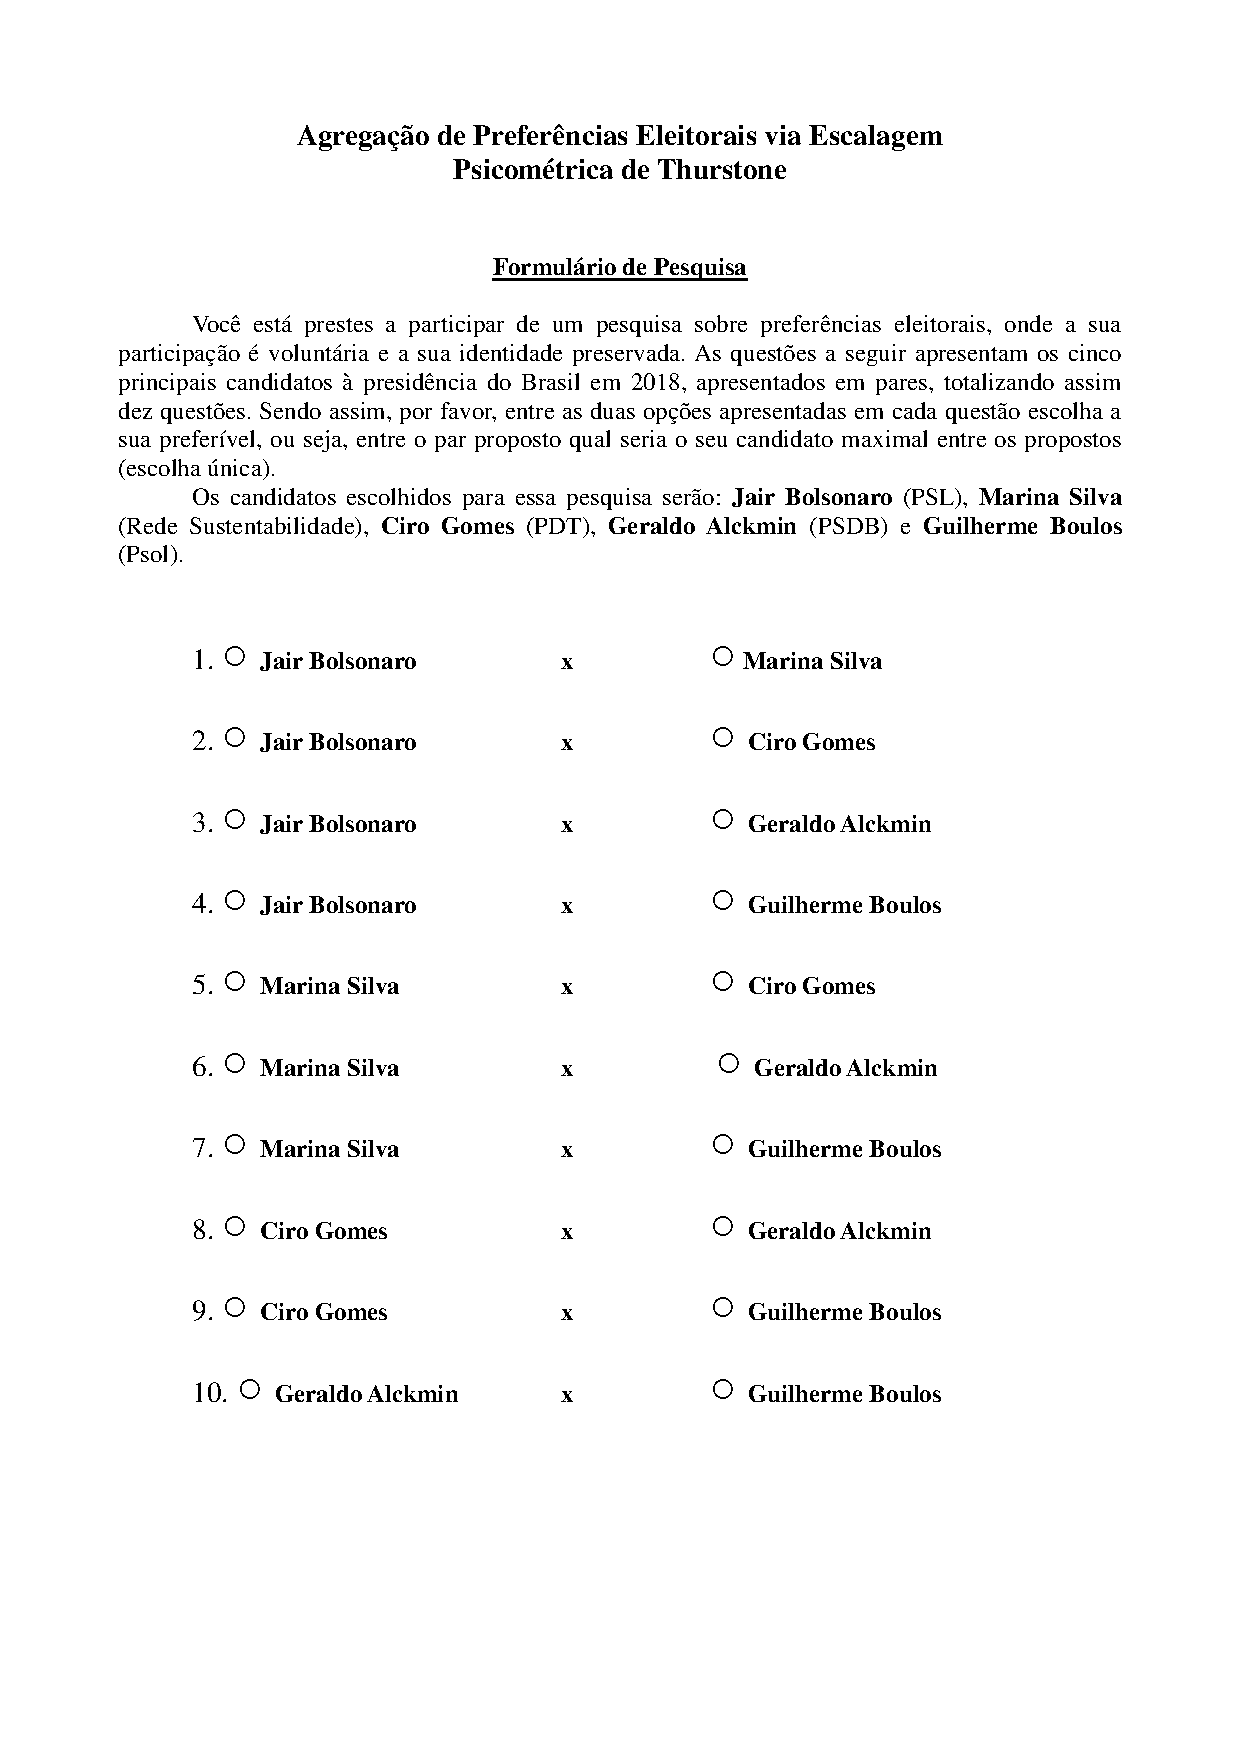
\includepdf[scale=0.8,pages=1,pagecommand=\chapter{Questionário}]{questionario.pdf}
%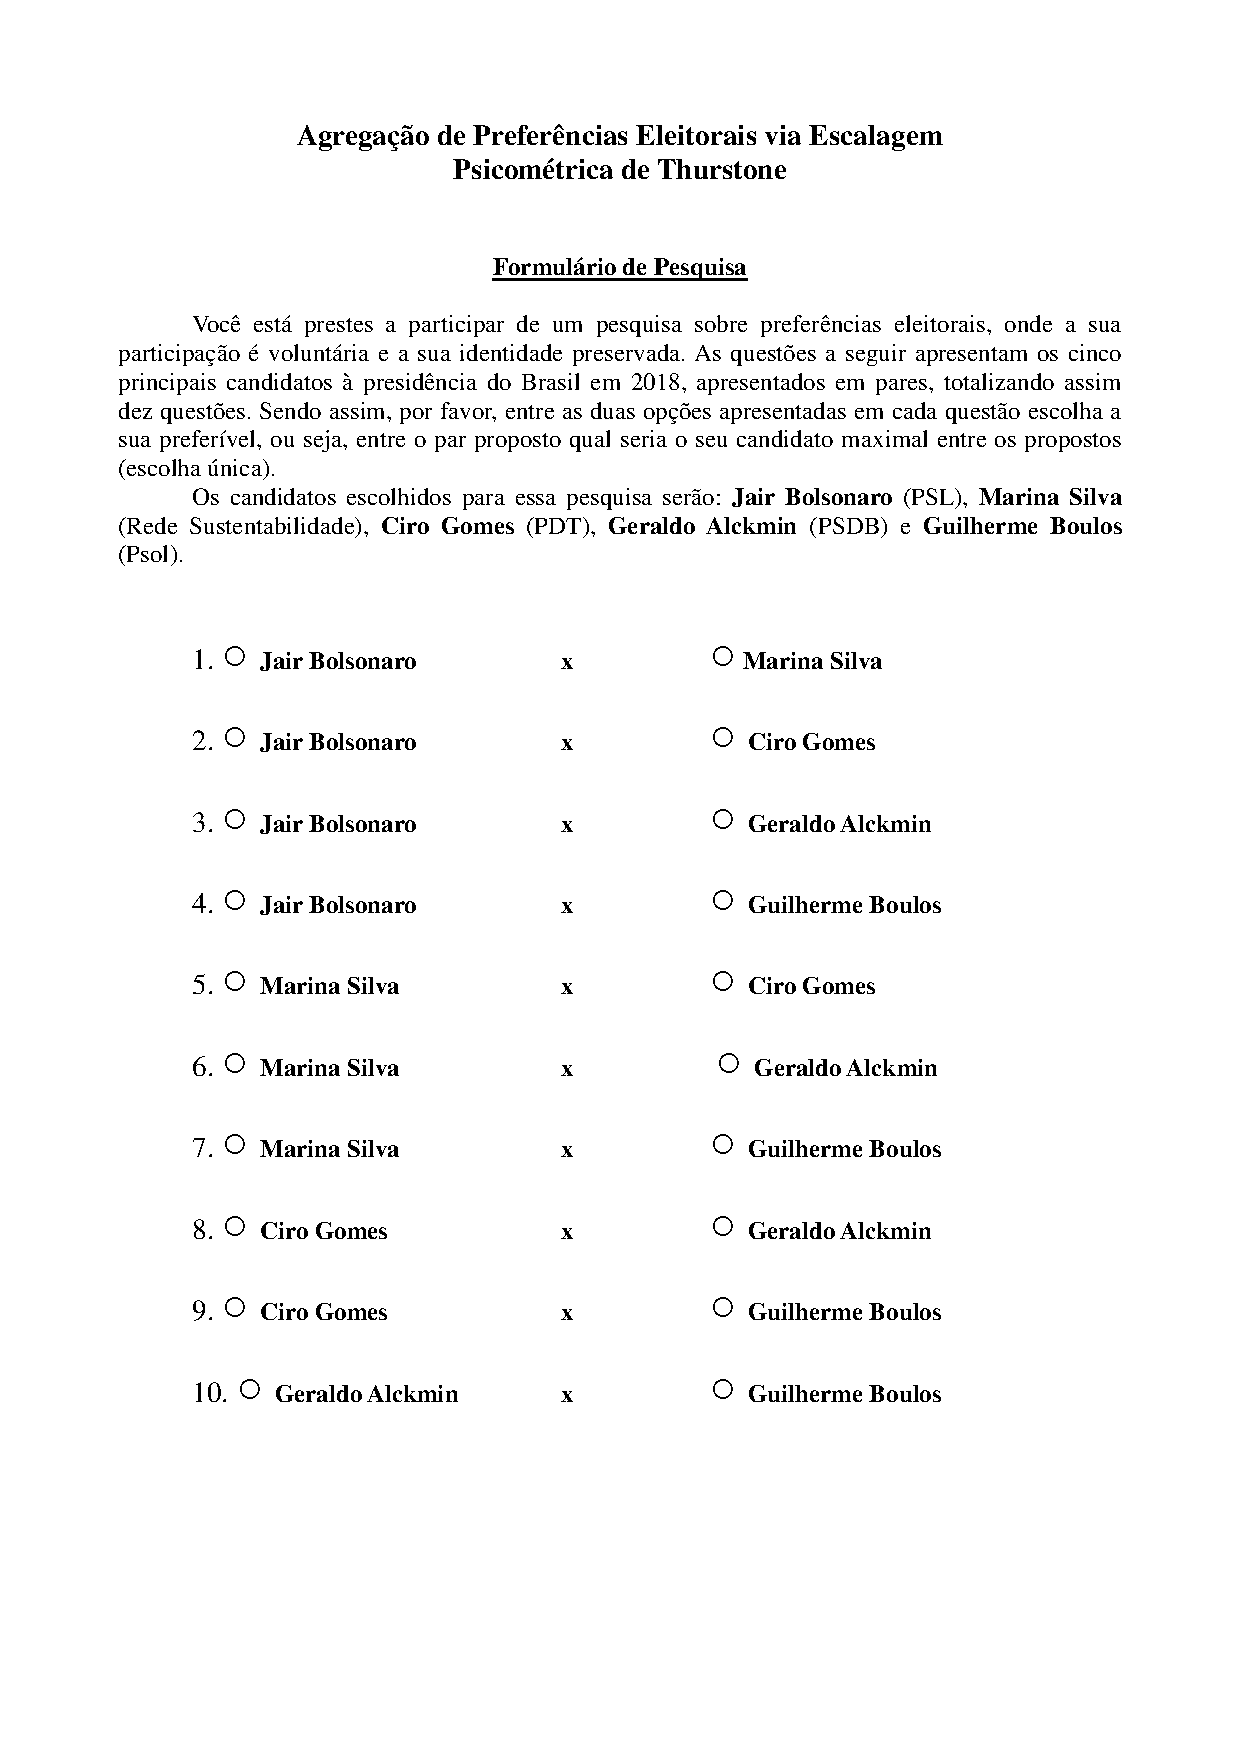
\includepdf[pages=1]{questionario.pdf}

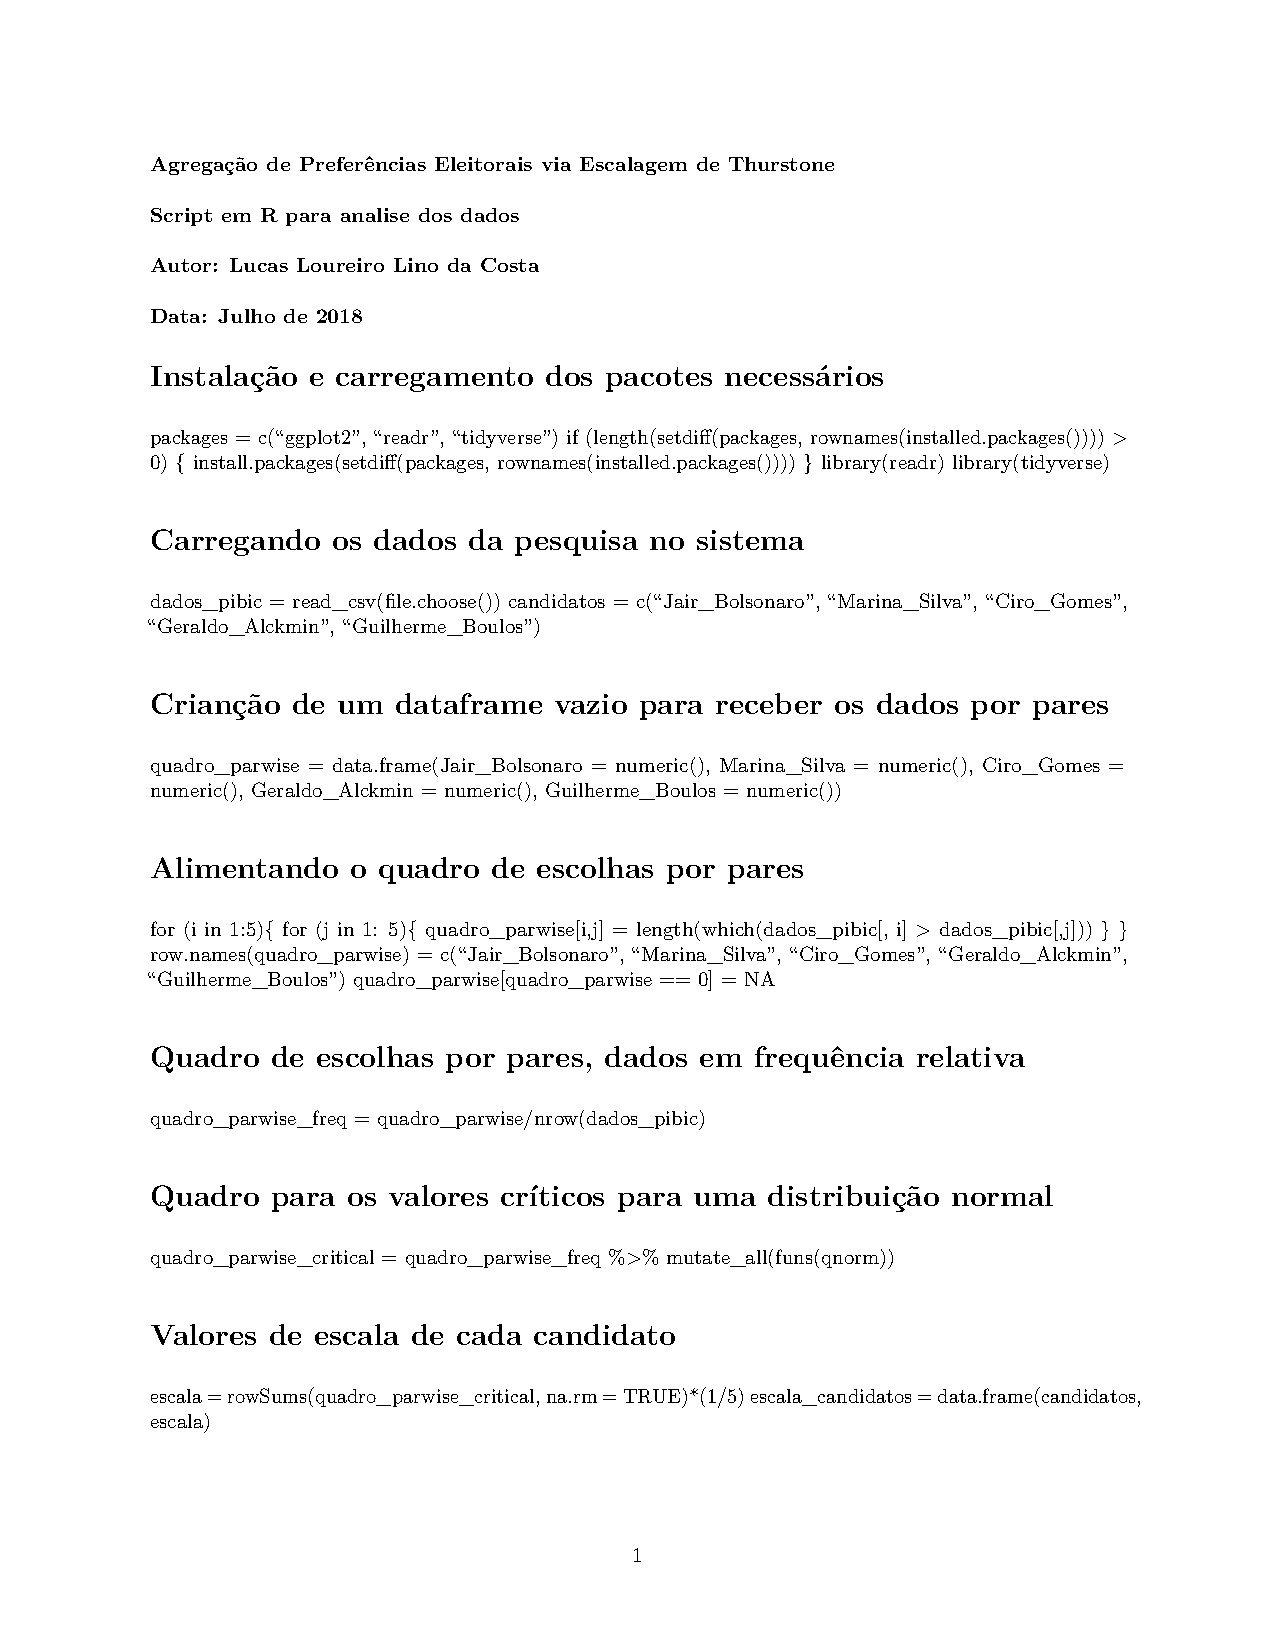
\includepdf[scale=0.8,pages=1,pagecommand=\chapter{R Script}]{script.pdf}
%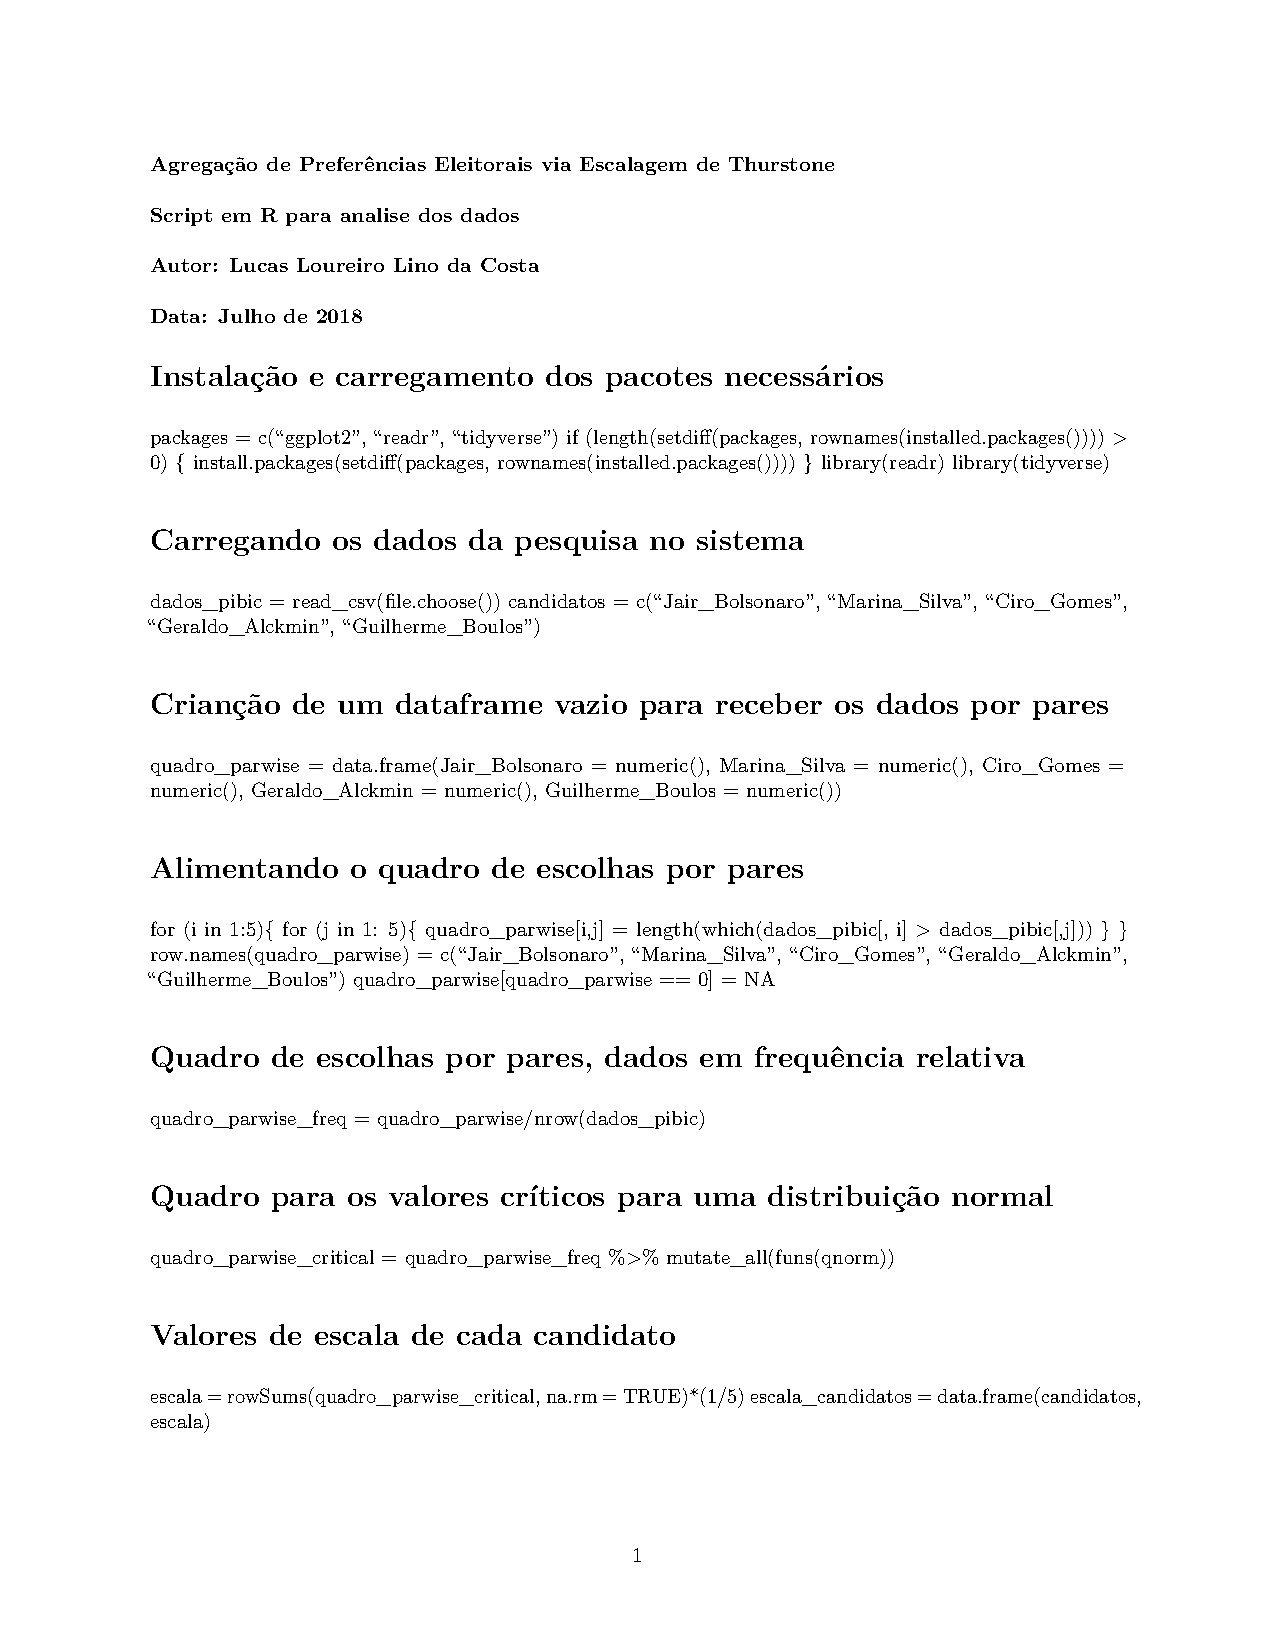
\includepdf[pages=1]{script.pdf}

\end{anexosenv}


% ----------------------------------------------------------
% Título e resumo em língua estrangeira
% ----------------------------------------------------------

% \twocolumn[    		% INICIO DE ARTIGO EM DUAS COLUNAS

% titulo em inglês
\titulo{Agregação de Preferências Eleitorais via Escalagem Psicométrica de Thurstone}
\emptythanks
\maketitle

% resumo em português
\renewcommand{\resumoname}{Abstract}
\begin{resumoumacoluna}
 \begin{otherlanguage*}{english}
In this work we will use an unusual method of dealing with ordinal categorical data in economic sciences, Thurstone's method of psychometric scaling. We will use it to determine aggregate preferences about candidates in elections from individual manifestations about pairs of alternatives. As an instance of application of the method, we will take a plausible list of candidates for the 2018 Brazilian presidential election, as well as a representative sample of the Faculty of Administration, Accounting and Economics of the University of Brasília, in order to infer the collective preferences of the population in question.

   \vspace{\onelineskip}
 
   \noindent
   \textbf{Key-words}: Collectives Aggregated Preferences. Unidimensional Psychometric Scale. Thurstone's method. Brazilian's Election 2018.
 \end{otherlanguage*}  
\end{resumoumacoluna}

% ]  				% FIM DE ARTIGO EM DUAS COLUNAS
% ---

\end{document}
